\documentclass{oci}
\usepackage[utf8]{inputenc}
\usepackage{lipsum}

\title{Rotar}
\codename{rotar}

\begin{document}
\begin{problemDescription}

  \centerline{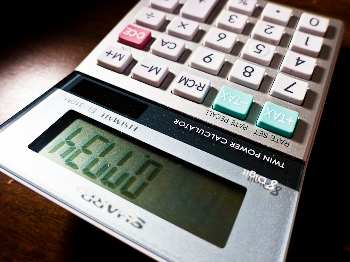
\includegraphics[scale=0.5]{upside-down.jpg}}


Camilo y Mauricio compran siempre en el mismo almacén de la esquina de su casa. %, el almacén de Objetos Caros e Inservibles (OCI).
Compran pan, queso, yoghurt, bebidas, etc. 
La vendedora, al otro lado del mesón, tiene una tremenda calculadora que usa para sacar las cuentas. 
Apreta botones, opera valores, y al final el total queda en el visor de la calculadora, 
desde donde Camilo y Mauricio leen cuánto tienen que pagar.

Camilo siempre se molesta en silencio pues la vendedora nunca se da el tiempo de girar la calculadora para que ellos puedan ver el monto.
Pero esta vez, caminando de regreso a casa, Camilo explotó.

---\emph{¡Odio tener que girar el número mentalmente para saber cuánto pagar!} ---expresó molesto Camilo, a lo que Mauricio respondió: \\
---\emph{Yo no me hago problemas. La mayoría de las cantidades mantienen su valor si las giras en 180 grados. Así que simplemente pago lo que leo en la calculadora desde nuestro lado.} \\
-- \emph{¡¿Qué?!} ---gritó espantado Camilo.

Para apoyar su punto, Mauricio menciona como ejemplo los números 906, 26592 y 18181, que en su versión original y al rotarlos en 180 grados (como si giraras el visor de la calculadora) se leen exactamente igual. La siguiente figura confirma lo dicho por Mauricio.

\bigskip
\bigskip

\begin{center}
\resizebox{!}{40pt}{\input{906.pspdftex}} \hspace*{50pt}  
\resizebox{!}{40pt}{\input{26592.pspdftex}} \hspace*{50pt}  
\resizebox{!}{40pt}{\input{18181.pspdftex}}\bigskip

{Figura 1: Cantidades que mantienen su valor al rotar la calculadora. Si no lo crees, gira esta hoja.}
\end{center}

\bigskip
\bigskip


Camilo por el contrario dice que hay muchos más números que no se verán iguales después de girar la calculadora
y no entiende qué montos ha pagado Mauricio cada vez.
Camilo da como ejemplo los números 999, 5128 y 379009 que no cumplen lo dicho por Mauricio, como se ve en la siguiente figura.

\bigskip
\bigskip

\begin{center}
\resizebox{!}{40pt}{\input{999.pspdftex}} \hspace*{50pt}  
\resizebox{!}{40pt}{\input{1835.pspdftex}} \hspace*{50pt}  
\resizebox{!}{40pt}{\input{379009.pspdftex}}\bigskip

{Figura 2: Cantidades que NO mantienen su valor al rotar la calculadora.}
\end{center}

\bigskip
\bigskip


La discusión llevó a una pelea interminable camino a casa, Mauricio diciendo que la vida es linda y no hay para qué estresarse, 
Camilo molesto pensando en toda las veces que Mauricio pagó el monto incorrecto, o simplemente un monto sin sentido. 
Decidieron que mejor no peleaban más y hacían un programa que verificara lo que decía cada uno.
Tu tarea entonces es hacer un programa que reciba una secuencia de dígitos que se escribieron en la calculadora y 
verifique si al rotar la calculadora en 180 grados el valor que queda es igual al inicial, como dice Mauricio, o si 
este cambia, como dice Camilo.

  
%  la prueba es con calculadora, y en lugar de utilizarla para sus cálculos, 
%  están decididos a usarla para hacer trampa. Para eso, le pasarán una calculadora a su amigo Jorgito, el mateo de la clase quién les dará las respuestas a través de la calculadora...\\
%
%  Pero ¿cómo podrán hacerlo ? ¡La respuesta está en el techo! En el techo de la sala hay un espejo, y a través de él Wax y Camilo podrán ver la calculadora de Jorgito. \\

%  \textit{Pero el espejo va a dar vuelta el número, y se verá rotado en 180 grados!} dice Camilo. Wax le dice que no se preocupe, que la mayoría de los números quedan iguales después de rotarlos en 180 grados. Como por ejemplo el 69 y el 25.\\
%
%  Camilo no le cree, ya que hay números como el 12 o el 37 que al rotarlos en 180 grados cambian. Así deciden apostar un centella para ver quién tiene razón.\\
%
%  Tu tarea es hacer un programa que reciba un número y verifique si al rotarlo en 180 grados queda igual o no.

\end{problemDescription}

\begin{inputDescription}
La entrada consiste en dos líneas. La primera contiene un entero $N$ que representa a la cantidad de dígitos que se escribieron en la calculadora y la segunda contiene $N$ números separados por un espacio, correspondiente a cada uno de los dígitos escritos en la calculadora.
\end{inputDescription}

\begin{outputDescription}
La salida consiste en una sola línea, la cuál debe tener una de dos palabras: \texttt{Mauricio} ó \texttt{Camilo}, dependiendo
de cuál de los dos tiene la razón para el número indicado.
\end{outputDescription}

\begin{scoreDescription}
  \score{10} $ N = 1$
  \score{10} $ N = 2$
  \score{10} $ N = 3$
  \score{20} $ 4 \leq N < 10$
  \score{20} $ 10 \leq N < 100$
  \score{30} $ 100 \leq N < 10000$
\end{scoreDescription}

\begin{sampleDescription}
\sampleIO{sample-1}
\sampleIO{sample-2}
\sampleIO{sample-3}
\sampleIO{sample-4}
\end{sampleDescription}

\end{document}
